\documentclass[a4paper,12pt]{article}
\fontfamily{book antiqua}
\usepackage{graphicx}
\usepackage{amsmath}
\usepackage{amsfonts}
\usepackage{amssymb}
\textwidth 15cm
\textheight 23cm
%\oddsidemargin -0.0in
%\oddsidemargin -10 true pt 

\begin{document}
\begin{titlepage}
\begin{center}

\begin{Huge}PyMorph\end{Huge}

\begin{large}
%[Python MORphological Parameters Hunter]
\end{large}
\vspace{5cm}
\begin{center}
Authors\end{center}
\vspace{0.5cm}
\begin{Large}Vinu Vikram, Yogesh Wadadekar, Ajit K. Kembhavi \end{Large}

\vspace{5cm}
2008
\end{center}
\end{titlepage}
\tableofcontents
\clearpage
\section{PyMorph}
{\bf PyMorph} is a pipeline, which gives non-parametric and parametric quantities in an automated way. PyMorph uses GALFIT (Peng et. al. 2002) for bulge disk decomposition of galaxy and SExtractor (Bertin et. al. 1996) for determining the initial values. PyMorph uses its own module to calculate the CASGM parameters. In this section I will explain the PyMorph in detail.
\subsection{Dependencies}
\begin{enumerate}
 \item Python 2.4 or greater
 \item Stsci$\_$python (This package includes numpy, pyfits, pyraf)
 \item GALFIT
 \item SExtractor
 \item matplotlib
 \item xpa (optional, if you want to select psf)
\end{enumerate}

\subsection{Working modes}
The pipeline will work in different modes. They are described shortly as follows.

\subsubsection{Normal Mode}
In normal mode, user will be able give two kind of inputs
\begin{itemize}
\item 
a. Galaxy(ies) in a large field
\item
b. Galaxy(ies) in cutout image(s)
\end{itemize}

\subsubsection{Repeat Mode}
\begin{itemize}
 \item 
The fitting process can be failed due to several reasons. If we feel the fitting can be improved by adjusting the initial values or using an efficient mask, this mode can be used.
\end{itemize}

\subsubsection{Find and Fit}
\begin{itemize}
\item 
Fit objects with in some magnitude range.
\end{itemize}
\subsubsection{Psf Selection}
\begin{itemize}
\item 
a. Run PyMorph to find and extract psf from the image
\item
b. Find psf and run PyMorph
\end{itemize}
\subsection{Pre-Pipeline Procedure}
\begin{enumerate}
 \item 
Run SExtractor on the frame and the resulting file contains the information of all the object in the frame. The output parameters of this MUST follow a particular order and that can be found in the appendix. This process is recommended, as the PyMorph may keep the sky value at the SExtractor value during the decomposition. So running SExtractor needs care. In case if the PyMorph does not find any SExtractor catalogue it will make one using the default parameters.
\item
Make a file which contains the position, redshift information etc. of the galaxies which we are going to fit.
\item
Make psf. Either using PyMorph or by some other means
\item
Edit the config.py which the configuration file for the pipeline. The parameters in the configuration file are described below
\end{enumerate}

\subsection{Input parameters}
\begin{itemize}
\item \textbf{imagefile:}
\begin{itemize}
\item[] The frame contains the galaxies. This will use only if you are decomposing galaxies in a large frame.
\end{itemize}

\item \textbf{whtfile:}
\begin{itemize}
\item[] The corresponding rms weight map of the large frame. If this file is not found the program will skip this step.
\end{itemize}

\item \textbf{sex\_cata:}
\begin{itemize}
\item[] The SExtractor catalogue of all the objects in the frame. If the user provide one SExtractor catalogue, PyMorph uses it. Otherwise it generate using the default SExtractor parameters. One can use the command line option \textit{--edit-conf} to change these parameters according to their images.
\end{itemize}

\item \textbf{clus\_cata:}
\begin{itemize}
\item[] The list of all the obects of interest. The possible columns in this file in the Section: \ref{cluscat} and each column should have the title. The program need atleast gal\_id or gimg to run.
\end{itemize}

\item \textbf{out\_cata:}
\begin{itemize}
\item[] The name of the output catalogue. This file is used to write all the galaxies detected by the program during the run.
\end{itemize}

\item \textbf{rootname}
\begin{itemize}
\item[] Root name. You can give just a blank '' to avoid using this. If you give a root name all the intermediate files and the name of the galaxy in the result file will be appended with this.
\end{itemize}

\item \textbf{psfselect}
\begin{itemize}
\item[] Since selecting GOOD psf and make a list of them is difficult, we have added a small utility which will help the users to find the psf with out spending much time. This can be achived by using the psfselect parameter. This parameter can take either 0, 1 or 2. The three possibilities are as follows
\begin{itemize}
\item 0 $=>$ No psf selection, ie. the pipeline will continue with the user supplied psfs.
\item 1 $=>$ Only Select psf. The pipeline will run only for selecting psfs.
\item 2 $=>$ Select psf and run pipeline.
\end{itemize}
\item[] It is recommended to use psfselect = 1 and select psf. After having
 good psf, continue pipeline run using psfselect = 0. If you are in hurry
 use psfselect = 2
\end{itemize}

\item \textbf{starsize}
\begin{itemize}
\item[] The size of the psf image in terms of the semi-major axis of the image. The size of the image will be\textit{ starsize * semi-major axis}
\end{itemize}

\item \textbf{psflist:}
\begin{itemize}
\item[] List of psfs. You can give it as a list like\textbf{ ['psf1.fts, 'psf2.fits', etc]} or give a file contains the psf name as\textbf{'@psflist.txt}'. The pipeline will select the nearest psf to the fitting galaxy either using the header or using the information from its name. If in the latter case, the psf's name should be in form\textbf{
 psf\_radec.fits}.
\begin{verbatim}Eg. If the psf's position is (12:16:43.5, -12:03:12.0) then the 
name should be psf_1216435-1203120.fits.
\end{verbatim}
\item[]  This convention is used to find the nearest psf. The pipline will first check whether the mode is repeat. If repeat is false and if the program fails to find the configuration file, then it will try to find the coordinate information of the galaxy. If the program doesn't find the RA and DEC information of the galaxy, then it chooses the psf one by one from the list.
\end{itemize}

\item \textbf{mag\_zero:}
\begin{itemize}
\item[] Magnitude Zero point.
\end{itemize}

\item \textbf{mask\_reg, thresh\_area, threshold:}
\begin{itemize}
\item[] Masking will start for neighbors whose distance from the object greater than threshold * semi-major axis of the object and area of the neighbor less than thresh\_area sq.pixel. The masking will be done for a circular region of radius mask\_reg * semi-major axis of the neighbor with respect to the center of the neighbour. In the case of large
 frame, it is possible that some light from objects from outside the cutout can also contaminate the cutout. In that case the program is intelligent enough to mask those region and elliptical masking will be used for those cases.
\end{itemize}

\item \textbf{size:}
\begin{itemize}
\item[] This parameter is a list of five parameters which controls the size and shape of the stamp image of the galaxy. The size parameters are in the order
\begin{verbatim}size = [resize, varsize, fracrad, square, fixsize]
\end{verbatim}

\item \textit{resize} - This will be used when the user supply a cutout and
 wishes to resize that image. This particular parameter is useful when
 we have a large number of individual galaxy images from surveys like
 SDSS.

\item \textit{varsize} - This parameter will be used to find the right image
 cutout size. When it is true the size of the image will be decided by
 using the half light radius.

\item \textit{fracrad} - The size of the image w.r.t. the half light radius.
 Size of the image will be\textit{ fracrad} times half light radius of the
 galaxy.

\item \textit{square} - This will decide whether the cutout is rectangular
 shaped or square shaped. For square shape, this will be 1.

\item \textit{ fixsize} - If the user wants to make an image of fixed size,
 this keyword will provide the size information.

\end{itemize}

\item \textbf{pixelscale}
\item \textbf{H0, WM, WV:}
\begin{itemize}
\item[] Hubble parameter, Omega matter, Omega lambda
\end{itemize}

\item The following parameters are used for calculating the CASGM parameters.
\begin{itemize}
\item[] \textbf{back\_extraction\_radius:}
\begin{itemize}
\item The radius of the background region
\end{itemize}
\item[] \textbf{angle:}
\begin{itemize}
\item The angle of rotation for the calculation of asymmetry
\end{itemize}

\end{itemize}

\item The following parameters decide the working mode of PyMorph
\begin{itemize}
\item[] \textbf{repeat:}
\begin{itemize}
\item Repeat the pipeline manually, if it is True
\end{itemize}

\item[] \textbf{galcut:}
\begin{itemize}
\item True if we provide cutouts
\end{itemize}

\item[] \textbf{decompose:}
\begin{itemize}
\item True, if you need 2D bulge disk decomposition
\end{itemize}

\item[] \textbf{cas:}
\begin{itemize}
\item True, if you need casgm parameters
\end{itemize}

\item[] \textbf{findandfit}
\begin{itemize}
\item '1', to use this mode otherwise '0'
\end{itemize}

\item[] \textbf{crashhandler}
\begin{itemize}
\item If it '1', then the PyMorph will handle the possible crashes and try to fix. The details can be found in the Section \ref{crash}
\end{itemize}

\end{itemize}

\item \textbf{components:} The user can decide the components for fitting. By default PyMorph will with a disk and a bulge to the object. The available componets are bulge, disk and point.
\item \textbf{fitting} This is also a list of three parameters which can be used to fix/fit center and sky.
\begin{verbatim} fitting = [bulge_center, disk_center, sky]
\end{verbatim}
The parameter are self explanatory.
\item The following parameters are used to classify good/bad fit.
\begin{itemize}
\item[] \textbf{chi2sq:}
\begin{itemize}
\item Good fit if the Chi2Nu $<$ chi2sq
\end{itemize}

\item[] \textbf{Goodness:}
\begin{itemize}
\item Good fit if the Goodness $>$ Goodness
\end{itemize}

\item[] \textbf{center\_deviation:}
\begin{itemize}
\item Good fit if abs(center - fitted center) $<$ abs(center - fitted center)
\end{itemize}

\end{itemize}

\end{itemize}
\subsection{config.py}
\begin{footnotesize}
\begin{verbatim}
"""Configure file for PyMorph. Authors: Vinu Vikram, Yogesh Wadadekar Ajit Kembhavi"""
###----Specify the input images and Catalogues----###
imagefile = 'j8f643-1-1_drz_sci.fits'
whtfile = 'j8f643-1-1_drz_rms.fits'  #The weight image. 
sex_cata = 'j8f643_sex.cat'          #The sextractor catalogue which has 
                                     #the format given in the file
clus_cata = 'cl1216-1201.cat'        #catalogue of galaxies from
                                     #online catalogu service
                                     #(name ra1 ra2 ra2 dec1 dec2 dec3)

###----Specify the output names of images and catalogues----###
out_cata = 'cl1216-1201_out.cat'     #catalogue of galaxies in the field
rootname = 'j8f643'

###----Psf list----###
psfselect = 0                        #0 => No psfselection
                                     #1 => Only Select psf 
                                     #2 => Select psf and run pipeline
                                     #Recommended: Run with '1' and then run
                                     #pipeline
starsize = 20                        #psf image size will be startsize times 
                                     #the SMA given by SExtractor
#psflist = ['psf_1216382-1200443.fits', 'psf_1216408-1200251.fits']
psflist = '@psflist.list'
                                     #List of psf containg their 
                                     #position information in the 
                                     #header (RA_TARG, DEC_TARG). 
                                     #Make psf with the names as here 
                                     #and use psf_header_update.py. 
                                     #It will update the header information.
mag_zero = 25.256                    #magnitude zero point

###----Conditions for Masking----###
manual_mask = 0
mask_reg = 2.0
thresh_area = 0.2
threshold = 3.0                      #Masking will be done for neighbours 
                                     #whose semimajor*threshold overlaps with 
                                     #threshold * semi-major axis of 
                                     #the object and area of the neighbour 
                                     #less than thresh_area * object area in
                                     #sq.pixel. 
                                     #The masking will be for a circular 
                                     #region of radius mask_reg*semi-major 
                                     #axis of the nighbour with respect to 
                                     #the center of the neightbour.
###---Size of the cut out and search conditions---###
###---size = [resize?, varsize?, fracrad, square?, fixsize]---###
size = [0, 1, 6, 1, 120]             #size of the stamp image
searchrad = '0.3arc'                 #The search radius  

###----Parameters for calculating the physical parameters of galaxy----###
pixelscale = 0.045                   #Pixel scale (arcsec/pixel)
H0 = 71                              #Hubble parameter
WM = 0.27                            #Omega matter
WV = 0.73                            #Omega Lambda

###----Parameters to be set for calculating the CASGM----###
back_extraction_radius = 15.0
#back_ini_xcntr = 32.0 
#back_ini_ycntr = 22.0
angle = 180.0

###----Fitting modes----###
repeat = False                       #Repeat the pipeline manually
galcut = False                       #True if we provide cutouts
decompose = True
galfit = True #Always keep this True as it is not functional yet!
cas = True
findandfit = 0
crashhandler = 1

###---Galfit Controls---###
components = ['bulge', 'disk']       #The components to be fitted to the objec
###---fixing = [bulge_center, disk_center, sky]
fitting = [1, 1, 0]                  # = 0, Fix params at SExtractor value

###----Set the SExtractor and GALFIT path here----###
GALFIT_PATH = '/home/vinu/software/galfit/modified/galfit' 
SEX_PATH = '/home/vinu/software/sextractor-2.5.0/sex/bin/sex'
PYMORPH_PATH = '/home/vinu/serial_pipeline/trunk/pymorph'

###----The following conditions are used to classify fit goo/bad----###
chi2sq = 1.9                         #< chi2sq
Goodness = 0.60                      #> Goodness
center_deviation = 3.0               #< abs(center - fitted center)
\end{verbatim}
\end{footnotesize}
\subsection{The parameters in clus\_cata}
\label{cluscat}
\begin{itemize}
\item \textbf{ gal\_id:} The identifier of the galaxy.
\item \textbf{ ra1, ra2, ra3:} The RA of the galaxy. ra1 is the degree part, ra2 is minute and ra3
 is the second part.
\item \textbf{ dec1, dec2, dec3:} The DEC of the galaxy and have same syntax as RAM
\item \textbf{ z:} The redshift of the galaxy
\item \textbf{ gimg:} The galaxy image
\item \textbf{ wimg:} The corresponding weight image
\item \textbf{ cfile:} Configuration file for GALFIT
\item \textbf{ ximg:} The x center of the galaxy
\item \textbf{ yimg:} The y center of the galaxy
\item \textbf{ bxcntr:} The x center of the background for finding the CASGM parameters
\item \textbf{ bycntr:} The y center of the background for finding the CASGM parameters
\item \textbf{ psf:} The psf corresponding to the galaxy
\item \textbf{ flag:} This will be used when the\textit{ crashhandler} is on. See the Flags section to know more.
\end{itemize}

\subsubsection*{Example clus\_cata}
The clus\_cata looks something like the following
\begin{footnotesize}
\begin{verbatim}
gal_id ra1 ra2 ra3 dec1 dec2 dec3 mag z bxcntr bycntr ximg yimg cfile psf flag
EDCSNJ1216453-1201176 12 16 45.26 -12 01 17.6 20.663 0.7955 20.0 20.0 60.0 60.0 
Gj8f647_EDCSNJ1216453-1201176.in psf_1216435-1203120.fits 128
\end{verbatim}
\end{footnotesize}
Another look
\begin{footnotesize}
\begin{verbatim}
gimg wimg ximg yimg bxcntr bycntr
Ij8f647_EDCSNJ1216453-1201176.fits Wj8f647_EDCSNJ1216453-1201176.fits 60.0 60.0 20.0 20.0
\end{verbatim}
\end{footnotesize}
The minimal clus\_cata
\begin{footnotesize}
\begin{verbatim}
gimg
Ij8f647_EDCSNJ1216453-1201176.fits
\end{verbatim}
\end{footnotesize}
Here we have assumed that the image \textit{Ij8f647\_EDCSNJ1216453-1201176.fit}s contains a galaxy within 10 pixels
 radius from the center. In the case of cut outs, the minimal configuration which uses all the PyMorph utilities is the following
\begin{footnotesize}
\begin{verbatim}
gimg z
Ij8f647_EDCSNJ1216453-1201176.fits 0.79
\end{verbatim}
\end{footnotesize}
\subsection{Command line Options}
Some command line options are also available and are explained as follows
\begin{itemize}
 \item 
\textbf{ --edit-conf (-e):} PyMorph use some default set of parameters to generate SExtractor catalogue. Since these input parameters affect the SEXtractor output and so the fit, the users are asked to make there own SExtractor  catalogue. This option allows the user to edit the SExtractor configuration file interactively.

\item
\textbf{ --force (-f): } Normally PyMorph will not generate SExtractor catalogue if it find one. Using this option user can generate SExtractor catalogue always.
\item
\textbf{ --with-psf: } By default, PyMorph will use the nearest psf from the psflist during decomposition. User can alter this behavior by this parameter. So \textit{--with-psf=0} takes the nearest psf, \textit{--with-psf=1} uses second nearest psf and soon. Using \textit{--with-psf=-1} one can use the farthest available psf. This will become particulary important in the case of testing psf variation over a large field / consistency of decomposition with psf.
\item
\textbf{ --help (-h): } Help on running pymorph with option
\item
\textbf{ --lmag}, \textbf{ --umag:} Minimum and maximum magnitudes allowed during fitting. By default lmag = 100 and umag = -100. Same range will be used for both bulge and disk.
\item
\textbf{ --ln}, \textbf{ --un: } The minimum and maximum allowed values of Sersic index. Defaults are 0.1 and 20.0.
\item
\textbf{ --lre},\textbf{ --ure: } Minimum and maximum allowed values of bulge scale length, re. Default 0 and 500 pixels.
\item
\textbf{ --lrd},\textbf{ --urd: } Minimum and maximum allowed values of disk scale length, rd. Default 0 and 500 pixels.
\item
\textbf{ --with-in: } Fitting will be done for objects which are NXPTS / 2 + with-in or NYPTS / 2 + with-in from the main object. By default it takes a value of 150. Usage: \textit{--with-in=150}.
\textbf{ --with-filter:} Manually give the filter. This will go to the database.
\textbf{ --with-db:} The MySQL database name.
\textbf{ --with-area:} The area of psf object.
\end{itemize}

\subsection{Working}
The architecture of the PyMorph is show in the figures and explained as follows

 \begin{figure}[tbh!]
 \centering
 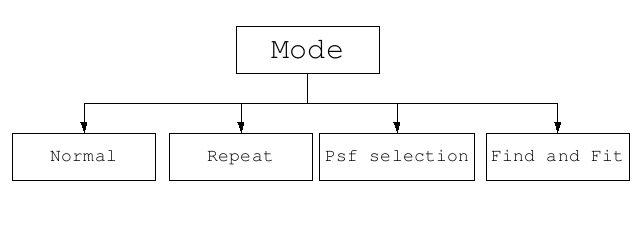
\includegraphics[width=8cm, height=3.5cm, bb=0 0 641 234]{pipeline-arch1.png}
 % pipeline-arch1.png: 641x234 pixel, 72dpi, 22.61x8.26 cm, bb=0 0 641 234
 \caption{The PyMorph Modes}
 \label{fig:arch1}
\end{figure}

\begin{figure}[tbh!]
 \centering
 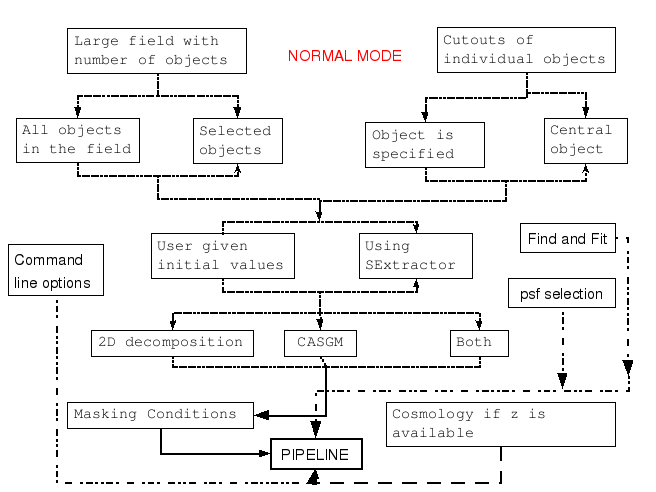
\includegraphics[width=11cm, height=8.5cm, bb=0 0 656 492]{pipeline-arch2.png}
 % pipeline-arch2.png: 656x492 pixel, 72dpi, 23.14x17.36 cm, bb=0 0 656 492
 \caption{PyMorph Architechture}
 \label{fig:arch2}
\end{figure}

\begin{figure}[tbh!]
 \centering
 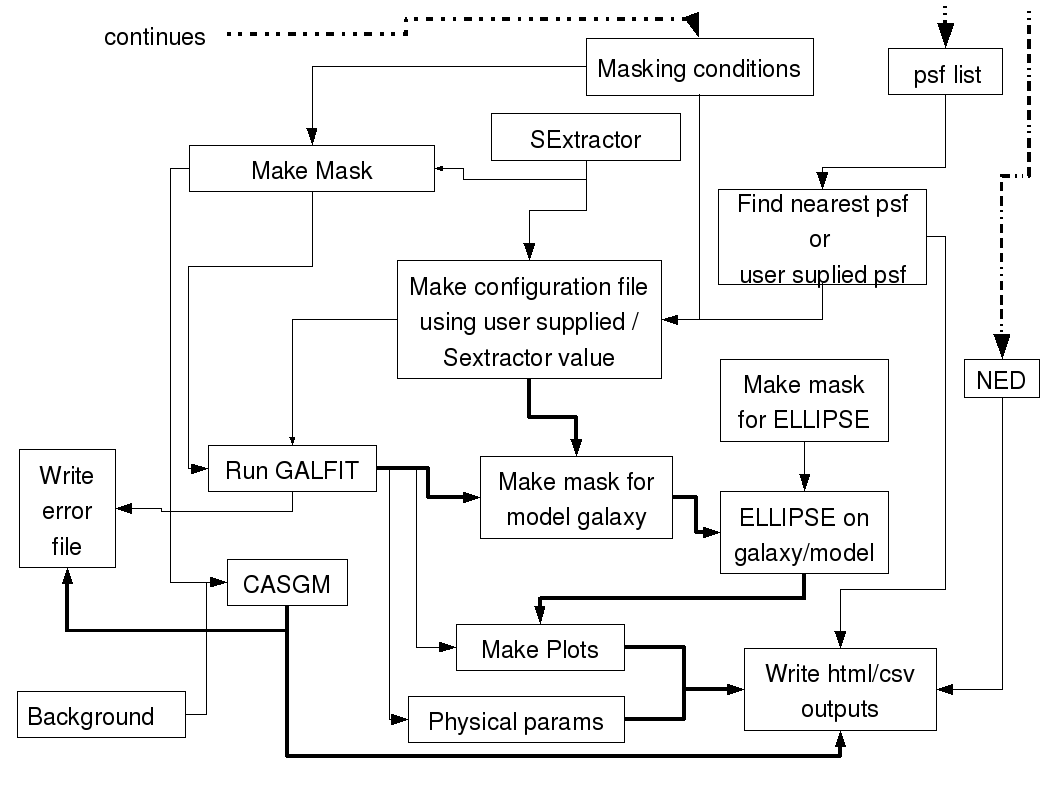
\includegraphics[width=11cm, height=8.5cm, bb=0 0 794 596]{pipeline-arch3.png}
 % pipeline-arch3.png: 1058x794 pixel, 96dpi, 28.00x21.01 cm, bb=0 0 794 596
 \caption{PyMorph Architecture}
 \label{fig:arch3}
\end{figure}

\begin{figure}[tbh!]
 \centering
 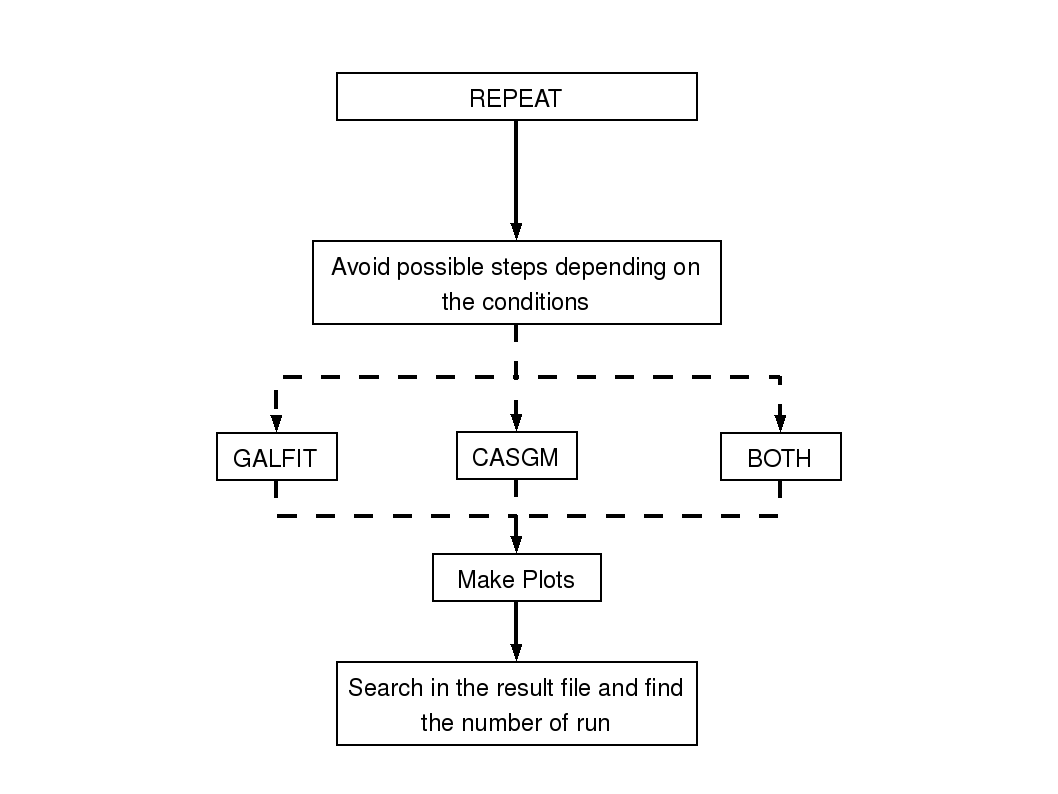
\includegraphics[width=11cm, height=8.5cm, bb=0 0 794 596]{pipeline-arch4.png}
 % pipeline-arch4.png: 1058x794 pixel, 96dpi, 28.00x21.01 cm, bb=0 0 794 596
 \caption{PyMorph Repeat Mode}
 \label{fig:arch4}
\end{figure}


\subsubsection{Normal Mode with large field}
\begin{itemize}
\item It compare the galaxy catalogue (clus\_cata) and sextractor catalogue (sex\_cata) and if the pipeline find an object in the sextractor catalogue, it will make a stamp image and the correspoding weight map of the galaxy. The pipline first try to match the RA and DEC information in clus\_cata with sextractor catalogue. If the clus\_cata doesn't have any of the ra1, ra2, ra3 and dec1, dec2, dec3 column, the pipeline will try to compare it with
 the physical coordinate of the object in the frame. So it will search for columns with headers ximg and yimg. If these colums are also unavailable the pipeline will not find any objects in the case of large frame and exit.
\item The pipeline will find the neighbour objects of the galaxy from the SExtractor catalogue.
\item It makes a mask using the parameters supplied in the configuration file.
\item It makes configuation file for running GALFIT using the SExtractor catalogue. Here the object will be fitted with Sersic + Exponential function and neighbours will be fitted by a single Sersic function.
\item Run GALFIT
\item Find the Physical parameters from the fitted one.
\item It makes a mask for Ellipse task. The mask for Ellipse task and that of GALFIT are different. In the case of Ellipse mask all objects near the galaxy will be masked and the pipeline will use the ellipticity and position angle information to do that. But in the case of the GALFIT mask a circular masking will be done according to the parameters
 supplied in the configuration file.
\item Run Ellipse task on the galaxy image using the SExtractor parameters as the initial values.
\item Run Ellipse task on the model image of the galaxy.
\item Compare the two 1-D profiles.
\item It makes plots of galaxy, model, residual, histogram, mask and the 1-D profiles.
\item It makes an html file and csv file contains the fitted parameters and casgm parameters.
\end{itemize}
\subsubsection{Normal Mode with cutouts}
 In this case also the pipeline does all the works as explained in the previous section. In addition to those, if you are supplying cutouts of galaxies, then the pipeline assumes the center of the object lies in the center of the cutout and assign the values of ximg and yimg as size/2.
\subsubsection{Repeat Mode}
In this mode, the pipeline assumes there is cutout of galaxies and it has made during the previous run. So if the clus\_cata contains the colums gimg or gal\_id, the pipeline runs for that galaxies. During this mode the pipeline will not make/alter any mask image and galfit configuration file, if they exists. So one can adjust his GALFIT configuration file / masking before running the pipeline in the REPEAT mode.
\subsubsection{Find and Fit}
In this mode user can fit objects without creating clus\_cata. PyMorph will ask the user some necessary information like the magnitude range, redshift and the object classification probability and find the morphological
 parameters. The user must create psf before going to run in this mode.
\subsubsection{Psf Selection}
One of most difficult problem during the Morphological parameter estimation is to get good psf. Even in the case of PyMorph the situation won't differ much. But PyMorph is providing a very handy tool to select the psf out of the frame. As one the collaborator tells, this procedure is something like playing computer game. It is interesting but need much care. The keywords in config.py, \textit{'psfselect'} and \textit{'starsize'} are the controlling parameters of the mode. By default PyMorph will find the nearest psf from the psf list. This will cause some problem while you are using cut image, where you will have one psf corresponding to one galaxy. Taking this in to account PyMorph will update the clus\_cata with one psf to each galaxy under the column \textit{'psf'}.
\subsubsection{Crash Handler}
\label{crash}
If the parameter \textit{crashhandler} is on in the config.py, it will be invoked in three situations
\begin{itemize}
\item Galfit crashes or one of the bulge / disk parameter hits the limit
\begin{itemize}
\item[] Solution: Try to fit again with the following conditions
\begin{itemize}
\item Fix / free sky, if it is free / fix
\item Fix / free centers of bulge and disk, if the centers are found free / fix
\end{itemize}
\end{itemize}

\item Reduced chi square is large
\begin{itemize}
\item[] Solution: Fix / free centers of bulge and disk, if the centers are found free / fix
\end{itemize}

\item Fake center
\begin{itemize}
\item[] Solution: Fix centers of bulge and disk.
\end{itemize}
\end{itemize}
The schematic diagram of crash handle is as following
\begin{figure}
 \centering
 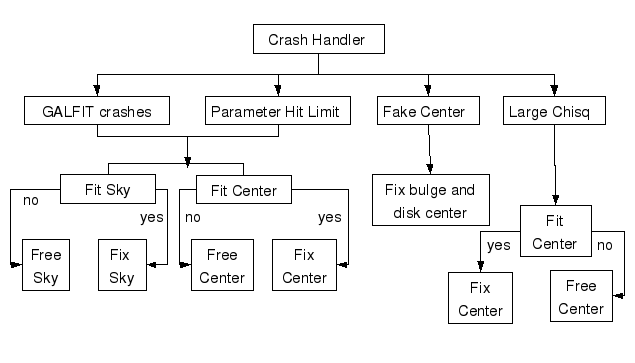
\includegraphics[width=10cm, height=5.7cm, bb=0 0 635 363]{pipeline-arch5.png}
 % pipeline-arch5.png: 635x363 pixel, 72dpi, 22.40x12.81 cm, bb=0 0 635 363
 \caption{Crash Handler}
 \label{fig:arch5}
\end{figure}

\subsection{Filenames}
The PyMorph will output a number of files and those filenames has adopted a unique format. The filename convention is illustrated below. Suppose in the config.py the parameter rootname = j8f645 and gal\_id, which is the name of the galaxy in the clus\_cata is 9999, then
\begin{itemize}
\item \textbf{Ij8f645\_9999.fits:} The cut out of the galaxy.
\item \textbf{Wj8f645\_9999.fits:} Correspoding weight image for the cuts.
\item \textbf{Mj8f645\_9999.fits:} Galfit mask.
\item \textbf{EMj8f645\_9999.fits:} for ellipse task.
\item \textbf{EMj8f645\_9999.fits.p:l} EMj8f645\_9999.fits will be converted to EMj8f645\_9999.fits.pl for
 ellipse task.
\item \textbf{Gj8f645\_9999.in:} Configuration file for GALFIT.
\item \textbf{Oj8f645\_9999.fits:} The ouput image from galfit.
\item \textbf{fit2.log:} The output parametrs will be append to this file
\item \textbf{error.log:} The process status of the pipeline can be seen in the file
\item \textbf{E\_j8f645\_9999.txt:} The ellipse task output of input image.
\item \textbf{OE\_j8f645\_9999.txt:} The ellipse task output of output image.
\item \textbf{P\_j8f645\_9999.png:} The plot of input, output, residue images and the 1-D profile comparison.
\item \textbf{R\_j8f645\_9999.html:} The html output including the figures and parameters.
\item \textbf{index.html:} The index file of all the fit will be in this.
\item \textbf{result.csv:} The csv file contains all the parameters
\item \textbf{agm\_result\_with\_radius.csv:} The file contains the radial variation of Asymmetry , Gini coefficients and M20
\item \textbf{restart.cat:} The catalogue contains all the objects with the corresponding lines in the clus\_cata. This catalogue can be used to restart the pymorph in the case of failed galaxies.
\item \textbf{CRASH.CAT:} Probably the user may not want to use this. This will be used in the case of crash handling.
\end{itemize}

\section{CASGM Description}

Concentration, Asymmetry, Clumpness, Gini coefficient and Moment of the galaxy (CASGM) are the quanties which have been used for the last few years to describe galaxy morphology and estimation of its evolution in the Non-parameteric way (Abraham et. al. 1996; Bershady et. al., Conselice et. al. 2003; Lotz et. al. 2004). We are describing the method we adopted to find these parameters in \textbf{PyMorph}.

\subsection{Concentration (C)}

1. It will find the radius $r_{\eta}$ where Petrosian parameter ($\eta$) is 0.2 The Petrosian parameter is defind as follows
\begin{equation}
\eta = \frac{L(R)}{L(<R)}
\end{equation}

L(R) is the light at a radius R and $L(<R)$ is the total light inside the radius R.

\begin{figure}[h]
\begin{center}
$\begin{array}{c@{\hspace{1cm}}c}
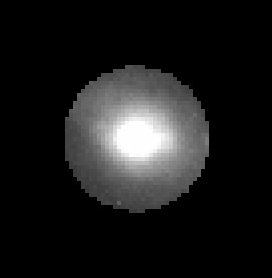
\includegraphics[width=4.5cm,height=4.5cm,bb=0 0 272 278]{C_r20.jpg}&
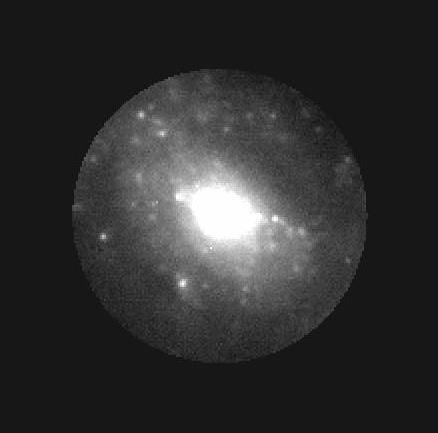
\includegraphics[width=4.5cm,height=4.5cm,bb=0 0 438 433]{C_r80.jpg}\\[0.1cm]
\mbox{20\% light contained portion} & \mbox{80\% light contained portion}
\end{array}$
\end{center}
\caption{Portion of galaxy within $r_{20}$ and $r_{80}$ }% \protect\ref{C and A}}
\label{Original and Rotated}
\end{figure}

2. Find the total light as the light inside $1.5 \times r_{\eta}$.

3. Find the $80\%$ and $20\%$ light contained radii. ie. $r_{80}$ and  $r_{20}$.

4. Find the concentration using the equation
\begin{equation}
C= 5 \log(\frac{r_{80}}{r_{20}})
\end{equation}

%\vspace{3cm}
\subsection{Asymmetry (A)}

1. Define an extraction region of radius $1.5 \times r_{\eta}$.

2. Rotating the image \footnote{The image used here is of NGC 5585 in R band.} by $180^0$

3. Find the asymmetry parameter using the equation
\begin{equation}
A = \frac{\sum\left|I_0 - I_\phi\right|}{2\sum |I_\phi|}
\end{equation}
where $I_\phi$ is the rotated image and $I_0$ is the original image.

4. Centering correction has been applied by minimizing the A value with center.

5. Noise correction has also been done by subtracting the asymmetry of the background from the image asymmetry.


\begin{figure}[h]
\begin{center}
$\begin{array}{c@{\hspace{1cm}}c@{\hspace{1cm}}c}
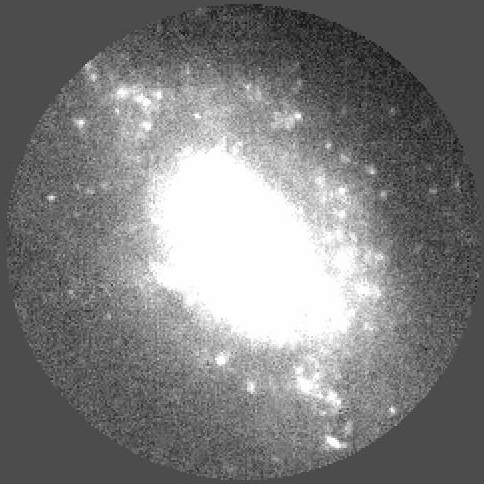
\includegraphics[width=4cm,height=4cm,bb=0 0 484 484]{original.jpg}&
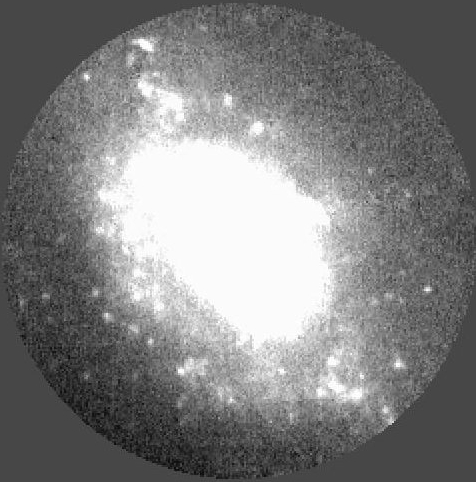
\includegraphics[width=4cm,height=4cm,bb=0 0 476 482]{rotated.jpg}&
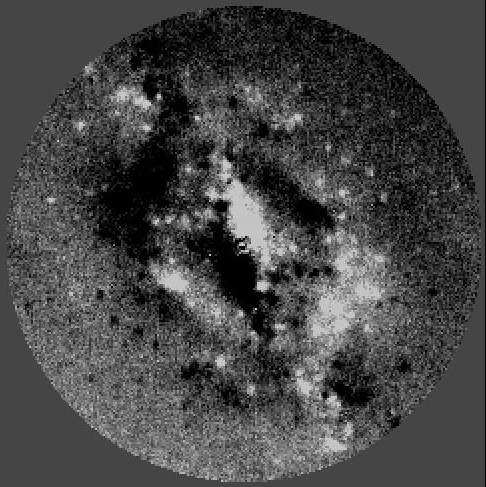
\includegraphics[width=4cm,height=4cm,bb=0 0 486 487]{residue.jpg}\\[0.1cm]
\mbox{Original image} & \mbox{Rotated image} & \mbox{Residual image}
\end{array}$
\end{center}
\caption{Images within the extraction radius}% \protect\ref{C and A}}
\label{Original and Rotated}
\end{figure}

\subsection{Clumpness (S)}

1. Smoothing the image with a boxcar of size $r_{\eta}/4$

2. Removing the center region of radius $r_{\eta}/4$, since the center region is not resolved.

3. Clumpness parameter can be computed using the equation
\begin{equation}
S = 10\times \frac{I - I^\sigma}{I}
\end{equation}

where I is the original image and $I^\sigma$ is the smoothed image.

4. Substract the background clumpness to get the final clumpness.

\begin{figure}[h]
\begin{center}
$\begin{array}{c@{\hspace{1cm}}c@{\hspace{1cm}}c}
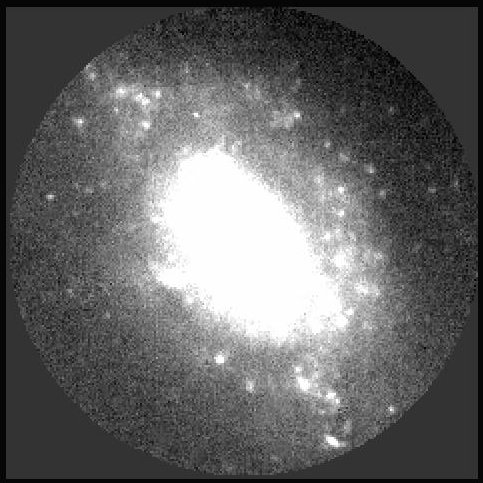
\includegraphics[width=4cm,height=4cm,bb=0 0 483 483]{ori_S.jpg}&
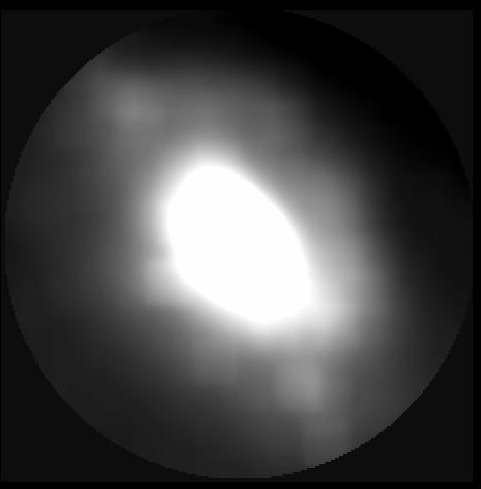
\includegraphics[width=4cm,height=4cm,bb=0 0 481 489]{smoothed.jpg}&
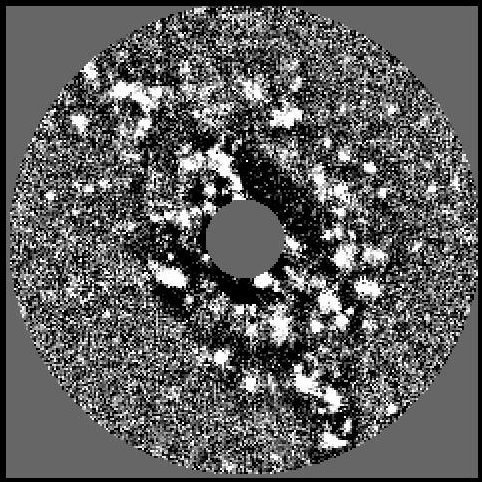
\includegraphics[width=4cm,height=4cm,bb=0 0 482 482]{res_S.jpg}\\[0.1cm]
\mbox{Original image} & \mbox{Smoothed image} & \mbox{Residual image}
\end{array}$
\end{center}
\caption{Images within the extraction radius}% \protect\ref{C and A}}
\label{Original Smoothed and Residual}
\end{figure}

\subsection{Gini coefficient (G)}
Gini coefficient tells how the galaxy light distributed among the pixels. Its value lie in between 0 and 1. If all the light is concentrated in one pixel, then G will be 1 and if all the light distributed uniformly among the pixels, then G will be zero.
1. Find the pixels in the image which belong to the galaxy, ie. make a segmentation map. This can be done by smoothing the image by a boxcar of size   $r_{\eta}/5$

2. The surface brightness at $r_{\eta}$, $\mu_{\eta}$ is measured and pixels in the smoothed image with flux values greater than $\mu_{\eta}$ and less than $10 \sigma$ is assigned to the galaxy. $\sigma$ is the sky deviation and it assures that any remaining cosmic rays or spurious noise pixels in the image are not  included in the segmentation map.

3. The Gini coefficient can be computed by the equation
\begin{equation}
G = \frac{1}{\overline{X} n (n-1)}\sum_{i}^n(2i-n-1)X_i
\end{equation}

 where the pixels in the segmentation map is sorted.

\begin{figure}[h]
        \centering
        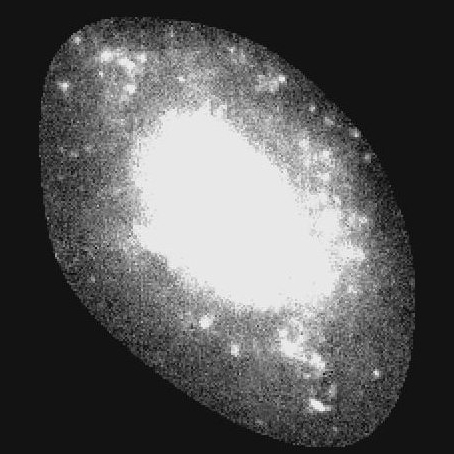
\includegraphics[width=4cm,height=4cm,bb=0 0 454 454]{segmentation.jpg}
% segmentation.jpg: 72dpi, width=22.54cm, height=16.97cm, bb=0 0 639 481
        \caption{Segmentation map of the galaxy}
        \label{fig:9}
\end{figure}

\subsection{The Moment of the Light (M20)}
1. The total second-order moment $M_{tot}$ is the flux in each pixel $f_i$ multiplied by the squared distance to the center of the galaxy, summed over all the galaxy pixels assigned by the segmentation map.
\begin{equation}
M_{tot}=\sum_{i}^n M_i=\sum_{i}^n f_i\left[ (x_i-x_c)^2 +(y_i-y_c)^2\right]
\end{equation}


where $x_c, y_c$ is the galaxy's center.

2. The center is computed by finding $x_c, y_c$ such that $M_{tot}$ is minimized.

3. Define $M_{20}$ as the brightest $20\%$ of the galaxy's flux.

4. To compute $M_{20}$, sort the pixels by flux, sum $M_i$ over the brightest pixels until the sum of the brightest pixels equals $20\%$  of the total galaxy flux, and then normalize by $M_{tot}$.
\begin{equation}
M_20 = \log\left( \frac{\sum M_i}{M_{tot}}\right)
\end{equation}

while $\sum_i f_i <0.2 f_{tot}$

5. $f_{tot}$ is the total flux of the segmentation map. The normalization by $M_{tot}$ removes the dependence  on total galaxy flux or size.
\section{2 dimensional Decomposition}
Two dimensional decomposition is the parametric way of describing galaxy light profile in terms of analytical functions. de Vaucouleurs (1948) observed that light profile of elliptical galaxy can be described by the analytical function
\begin{equation}
\Sigma(r) = \Sigma_e e^{-7.87 (\frac{r}{r_e})^{\frac{1}{4}}}
\end{equation}
In general, the bulge part of a galaxy can be modelled by Sersic(1968) function
\begin{equation}
 \Sigma(r) = \Sigma_e e^{-\kappa (\frac{r}{r_e})^{\frac{1}{n}}}
\end{equation}
where $\Sigma_e$ is the surface brightness of the galaxy at the effective radius $r_e$, $n$ is the Sersic index, $\kappa = 2n - 0.331$ is a function of $n$. The elegance of Sersic profile is that it gives de Vaucouleurs profile when $n = 1$  and exponential profile for $n = 1$, which is used to model the disk part of the galaxy.
\begin{equation}
\Sigma(r) = \Sigma_0 e^{-\frac{r}{r_d}}
\end{equation}
where $r_d$ is the disk scale length and $\Sigma_0$ is the central surface brightness.

\section{Methods}
\subsection{Masking}
In PyMorph masking will be done separately for ellipse task and for decomposition. In the case of ellipse task all the neighbors are masked using the SExtractor information. But SExtractor can be failed to resolve small objects near the brighter ones. In that case the PyMorph will try to find those using the following method.
\begin{itemize}
\item It will find the maximum value inside a small radius of the object
 of our interest.
\item It will search any other pixels out side the small radius above the
 maximum. If there are something it will mask mask those pixels. Then
 using that mask, the image will be masked. The central part where the
 maximum is found will also be masked. Then the radius will be increased
 further and again find the maximum inside that. This will continue till
 the image boundary.
\item If it doesn't find any pixels above the maximum, the program will
 increase the radius and go on.
\item After it reaches the image boundary, using the\textbf{ ndimage}\textit{
 fill\_hole} and\textit{ erosion} functions suitable operations on
 masking will be done. This will remove one pixel mask etc. In the case
 of masking for decomposition, only object which doens't fit will be
 masked.
\end{itemize}


\subsection{Sky Sigma and Background region}
If the user supply the background center, PyMorph will find the sky deviation from that region. But if these
 parameters are not given, then the Pymorph will calculate the sky deviation first and then using this find the background region. To find the sky deviation, the PyMorph will first mask all the object detected in the cutout. Then
 using that mask find the sky deviation. Since the estimation of CASGM parameters needs to know a background region of size \textit{back\_extraction\_radius} defind in the config.py. So the process is as follows
\begin{itemize}
\item Take an initial point ($\frac{back\_extraction\_radius}{2}$, $\frac{back\_extraction\_radius}{2}$) in the image.
\item Find the sky deviation within a region of radius \textit{back\_extraction\_radius}. If this deviation is less than the n * sky sigma (where n = 2 as starting value), take that region as background region, else go to the point ($\frac{back\_extraction\_radius}{2} + 2.0$, $\frac{back\_extraction\_radius}{2} + 2.0$).
\item The above process will go on till it reaches ($size - \frac{back\_extraction\_radius}{2}$ , $size - \frac{back\_extraction\_radius}{2}$) where size is the image size.
\item Still the result is negative, increase n from 2 to 3 and continue the process till we find the background region.
\item This process has disadvantage as it won't consider the gradient of sky.
\end{itemize}
\subsection*{Goodness}
It is defind as the ratio of number pixels within n times sky sigma around sky value to the total number of pixels.

\subsection{Flags}
The flags used in PyMorph are the following

\begin{center}
% use packages: array
\begin{tabular}{ll}
Flag & Explanation \\ 
1 & Repeat Mode \\ 
2 & Fit bulge center \\ 
4 & Fit disk center \\ 
8 & Fit sky \\ 
16 & The cutimage extend goes outside the image \\ 
32 & Galaxy ellipse failed \\ 
64 & Casgm failed \\ 
128 & Galfit failed \\ 
256 & Plotting failed \\ 
512 & Fitting bulge \\ 
1024 & Fitting disk \\ 
2048 & Fitting point \\ 
4096 & Neighbour fit \\ 
8192 & Large chisq  \\ 
16384 & Low goodness \\ 
32768 & Fake center \\ 
65536 & Sersic parameter hit the limit \\ 
131072 & Disk parameter hit the limit \\
262144 & Asymmetry is not Converged \\
524288 & Asymmetry calculation goes outside frame \\
1048576 & Background region determination is poor \\
\end{tabular}
\end{center}

\subsection{How to run PyMorph?}
\begin{itemize}
\item tar xzvf PyMorph.tar.gz
\item cp config.py /your/data/area/where/you/want/to/run/pymorph
\item Edit .cshrc file and give
\begin{footnotesize}
\begin{verbatim}
setenv PYTHONPATH /path/to/PyMorph/pymorph
alias pymorph '/path/to/PyMorph/pymorph.py'
\end{verbatim}
\end{footnotesize}
\item cd /your/data/area/where/you/want/to/run/pymorph
\item Edit config.py and add path to your GALFIT and SExtractor binaries.
\item pymorph [options]
\end{itemize}

\section{Appendix}
As you know SExtractor needs a configuration file, output parameters file, convolution kernel file and Neural Network file for Star/Galaxy classification files for its execution. 
PyMorph uses the following files as default.
\subsection{Parameter File}
\begin{footnotesize}
\begin{verbatim}
#-------------------------------- Catalog ------------------------------------
 
CATALOG_NAME     j8f631_sex.cat       # name of the output catalog
CATALOG_TYPE     ASCII_HEAD     # NONE,ASCII,ASCII_HEAD, ASCII_SKYCAT,
                                # ASCII_VOTABLE, FITS_1.0 or FITS_LDAC
PARAMETERS_NAME  default.param  # name of the file containing catalog contents
 
#------------------------------- Extraction ----------------------------------
 
DETECT_TYPE      CCD            # CCD (linear) or PHOTO (with gamma correction)
DETECT_MINAREA   6              # minimum number of pixels above threshold
DETECT_THRESH    1.5            # <sigmas> or <threshold>,<ZP> in mag.arcsec-2
ANALYSIS_THRESH  1.5            # <sigmas> or <threshold>,<ZP> in mag.arcsec-2
 
FILTER           Y              # apply filter for detection (Y or N)?
FILTER_NAME      default.conv   # name of the file containing the filter
 
DEBLEND_NTHRESH  32             # Number of deblending sub-thresholds
DEBLEND_MINCONT  0.005          # Minimum contrast parameter for deblending
 
CLEAN            Y              # Clean spurious detections? (Y or N)?
CLEAN_PARAM      1.0            # Cleaning efficiency
 
MASK_TYPE        CORRECT        # type of detection MASKing: can be one of
                                # NONE, BLANK or CORRECT
 
#------------------------------ Photometry -----------------------------------
 
PHOT_APERTURES   5              # MAG_APER aperture diameter(s) in pixels
PHOT_AUTOPARAMS  2.5, 3.5       # MAG_AUTO parameters: <Kron_fact>,<min_radius>
PHOT_PETROPARAMS 2.0, 3.5       # MAG_PETRO parameters: <Petrosian_fact>,
                                # <min_radius>
PHOT_FLUXFRAC    0.5            # flux fraction[s] used for FLUX_RADIUS
SATUR_LEVEL      100000.0        # level (in ADUs) at which arises saturation
MAG_ZEROPOINT    25.256            # magnitude zero-point
MAG_GAMMA        4.0            # gamma of emulsion (for photographic scans)
GAIN             1.0            # detector gain in e-/ADU
PIXEL_SCALE      0            # size of pixel in arcsec (0=use FITS WCS info)
 
#------------------------- Star/Galaxy Separation ----------------------------
 
SEEING_FWHM      0.11            # stellar FWHM in arcsec
STARNNW_NAME     default.nnw    # Neural-Network_Weight table filename
 
#------------------------------ Background -----------------------------------
 
BACK_SIZE        64             # Background mesh: <size> or <width>,<height>
BACK_FILTERSIZE  3              # Background filter: <size> or <width>,<height>
 
BACKPHOTO_TYPE   GLOBAL         # can be GLOBAL or LOCAL
 
#--------------------- Memory (change with caution!) -------------------------
 
MEMORY_OBJSTACK  3000           # number of objects in stack
MEMORY_PIXSTACK  300000         # number of pixels in stack
MEMORY_BUFSIZE   1024           # number of lines in buffer
 
#----------------------------- Miscellaneous ---------------------------------
 
VERBOSE_TYPE     NORMAL         # can be QUIET, NORMAL or FULL
WRITE_XML        N              # Write XML file (Y/N)?
XML_NAME         sex.xml        # Filename for XML output

#------------------------------ Check Image ----------------------------------

CHECKIMAGE_TYPE  APERTURES           # can be NONE, BACKGROUND, BACKGROUND_RMS,
                                # MINIBACKGROUND, MINIBACK_RMS, -BACKGROUND,
                                # FILTERED, OBJECTS, -OBJECTS, SEGMENTATION,
                                # or APERTURES
CHECKIMAGE_NAME  check.fits     # Filename for the check-image

#-------------------------------- WEIGHTing ----------------------------------

WEIGHT_TYPE      MAP_RMS           # type of WEIGHTing: NONE, BACKGROUND,
                                # MAP_RMS, MAP_VAR or MAP_WEIGHT
WEIGHT_IMAGE     j8f631_drz_rms.fits    # weight-map filename
WEIGHT_GAIN      N              # modulate gain (E/ADU) with weights? (Y/N)
\end{verbatim}
\end{footnotesize}
\subsection{Output Parameters}
\begin{footnotesize}
\begin{verbatim}
NUMBER
X_IMAGE
Y_IMAGE
ALPHA_SKY
DELTA_SKY
FLUX_ISO
FLUXERR_ISO
MAG_ISO
MAGERR_ISO
FLUX_RADIUS
BACKGROUND
THETA_IMAGE
ELONGATION
ISO0
A_IMAGE
FLAGS
CLASS_STAR
MAG_BEST           Uses in the case of findandfit mode
\end{verbatim}
\end{footnotesize}
\subsection{The Convolution Kernel}
\begin{footnotesize}
\begin{verbatim}
By default PyMorph uses 5x5 convolution mask of a Gaussian PSF with FWHM = 2.5 pixels.
\end{verbatim}
\end{footnotesize}
\subsection{Neural Netwrok}
\begin{footnotesize}
\begin{verbatim}
PyMorph uses the default.nnw file coming with SExtractor
\end{verbatim}
\end{footnotesize}
\end{document}
